\clearpage
\chapter{\textit{De L'Exp\'{e}rience}}
\label{ch:experience}

\textit{De L'Exp\'{e}rience} is a composition by Tod Machover in in
eight sections for narrator, organ, and electronics. The piece was
commissioned by the \textit{Orchestre Symphonique de Montr\`{e}al}
(OSM), and premiered at the \textit{Maison Symphonique de
  Montr\'{e}al} on May 16th, 2015. The text for the piece was taken
from the writings of Michel de Montaigne, the 16th century philosopher
known for popularizing the essay form.  Performers include Jean-Willy
Kunz, organist in residence with the OSM, and narrator, Gilles
Renaud. A recording of the performance is available
online.\sidenote{\url{http://web.media.mit.edu/~holbrow/mas/TodMachover_OfExperience_Premier.wav}}


\subsection{The Organ}
\label{sec:organ}
The project presented a unique challenge that fits well with the
themes in this thesis. The acoustic pipe organ can project sound into
space unlike any array of loudspeakers. This is especially true for an
instrument as large and magnificent as the Pierre B\'{e}ique Organ in
the OSM concert hall, which has 6489 pipes, and extends to
approximately 10 meters above the stage. Our objective is to blend
the sound of the organ with the sound of electronics. 
% The design of the organ is a collaboration between
% Diamond Schmitt Architects and Quebec-based organ manufacturer
% Casavant.

\section{Electronics}
\label{sec:electronics}
The electronics in the piece are a mix of synthesizers, pre-recorded
acoustic cello, and other processed material from acoustic and
electronic sources, all composed by Tod Machover. Prior to the
performance, these sounds were mixed ambisonically:
\begin{enumerate}
\item The cello was placed in front, occupying approximately the front
  hemisphere of our surround sound image.
\item The left and right channel of the electronic swells were panned
  to the left and right hemispheres. However, by default they were
  collapsed to omnidirectional mono (the sound comes from all
  directions, but has no stereo image). The gain of this synth was
  mapped to directionality, so when the synth grows louder, the left
  and right hemisphere become distinct from each other, and it create
  an illusion as if the sound is growing larger.
\item Additional sound sources are positioned in space such that each
  has as wide an image as possible, but overlaps with others as little
  as possible.
\end{enumerate}
The overarching goal of this approach was to create a diverse but
interesting spatial arrangement, but keep sounds mostly panned in the
same spot. Movement will be created by the warping of the surround
image by the Hypercompressor.

\subsection{Sound Reinforcement}
\label{sec:sound-reinforcement}
Loudspeakers were positioned throughout the hall. A number of factors
went into the arrangement: audience coverage, surround coverage,
rigging availability, and setup convenience. All speakers used were by
Meyer Sound.\sidenote{\url{http://www.meyersound.com/}} A single CQ-2
was positioned just behind and above the narrator, to help localize
the image of his voice.  JM-1P speakers on stage left and and stage
right were also used for the voice of the narrator, and incorporated
into the ambisonic playback system. Ten pairs of UPJ-1Ps were placed in
the hall, filling in the sides and rear for ambisonic playback, Two at
the back of the hall, mirroring the CQ-2s on stage, four on each of
the first and third balconies.  The hall features variable acoustics,
and curtains can be drawn into the hall to increase acoustic
absorption, and decrease reverb time. These were partially engaged,
striking a balance: The reduced reverb time improved the clarity of
amplified voice, while only marginally impacting the beautiful
acoustic decay of the organ in the hall. The show was mixed by Ben
Bloomberg. Ambisonic playback and multitrack recording of the
performance was made possible with the help and expertise of Fabrice
Boissin and Julien Boissinot and the Centre for Interdisciplinary
Research in Music Media and Technology (CIRMMT) at McGill University.

\paragraph{A note on composition, performance, and engineering}
No amount of engineering can compensate for poor composition,
orchestration, or performance. A skilled engineer with the right tools
only can only mitigate shortcomings in a performance. Good engineering
starts and ends with good composition, arrangement and performance. I
am have been quite fortunate that all the musicians involved with
\textit{De L'Exp\'{e}rience} at every stage are of the highest
caliber.

\section{Live Hypercompression Technique}
\label{sec:live-hyperc-techn}
During the performance, the encoded ambisonic electronic textures were
patched into the main input of the Hypercompressor, before being
decoded in realtime using the \textit{Rapture3D Advanced} ambisonic
decoder by Blue Ripple
Sound.\sidenote{\url{http://www.blueripplesound.com/products/rapture-3d-advanced}}
Four microphones captured the sound of the organ: Two inside, and two
hanging in front. The placement of the mics was intended to capture as
much of the sound of the organ as possible, and as little of the sound
of the amplified electronics in the hall. These four microphone
signals where encoded to ambisonics in realtime, and the resulting
ambisonic feed was patched into the side-chain input of the
Hypercompressor. In this configuration, the organ drives the
spatialization of the electronic sounds. By ambisonically panning the
organ microphones, we can control how our electronics are
spatialized. After some experimentation we discovered the best way to
apply the Hypercompressor in the context of \textit{De
  L'Exp\'{e}rience}. When the organ was played softly, the sound of
the electronics fills the performance hall from all directions. As the
organ plays louder, the electronic textures dynamically warp toward
the organ in the front of the concert hall. The spatial and timbral
movement of the electronics together with the magnificent (but stable)
sound of the the organ create a unique blend that is inaccessible with
acoustic or electronic sounds in isolation.

\begin{figure*}[]
  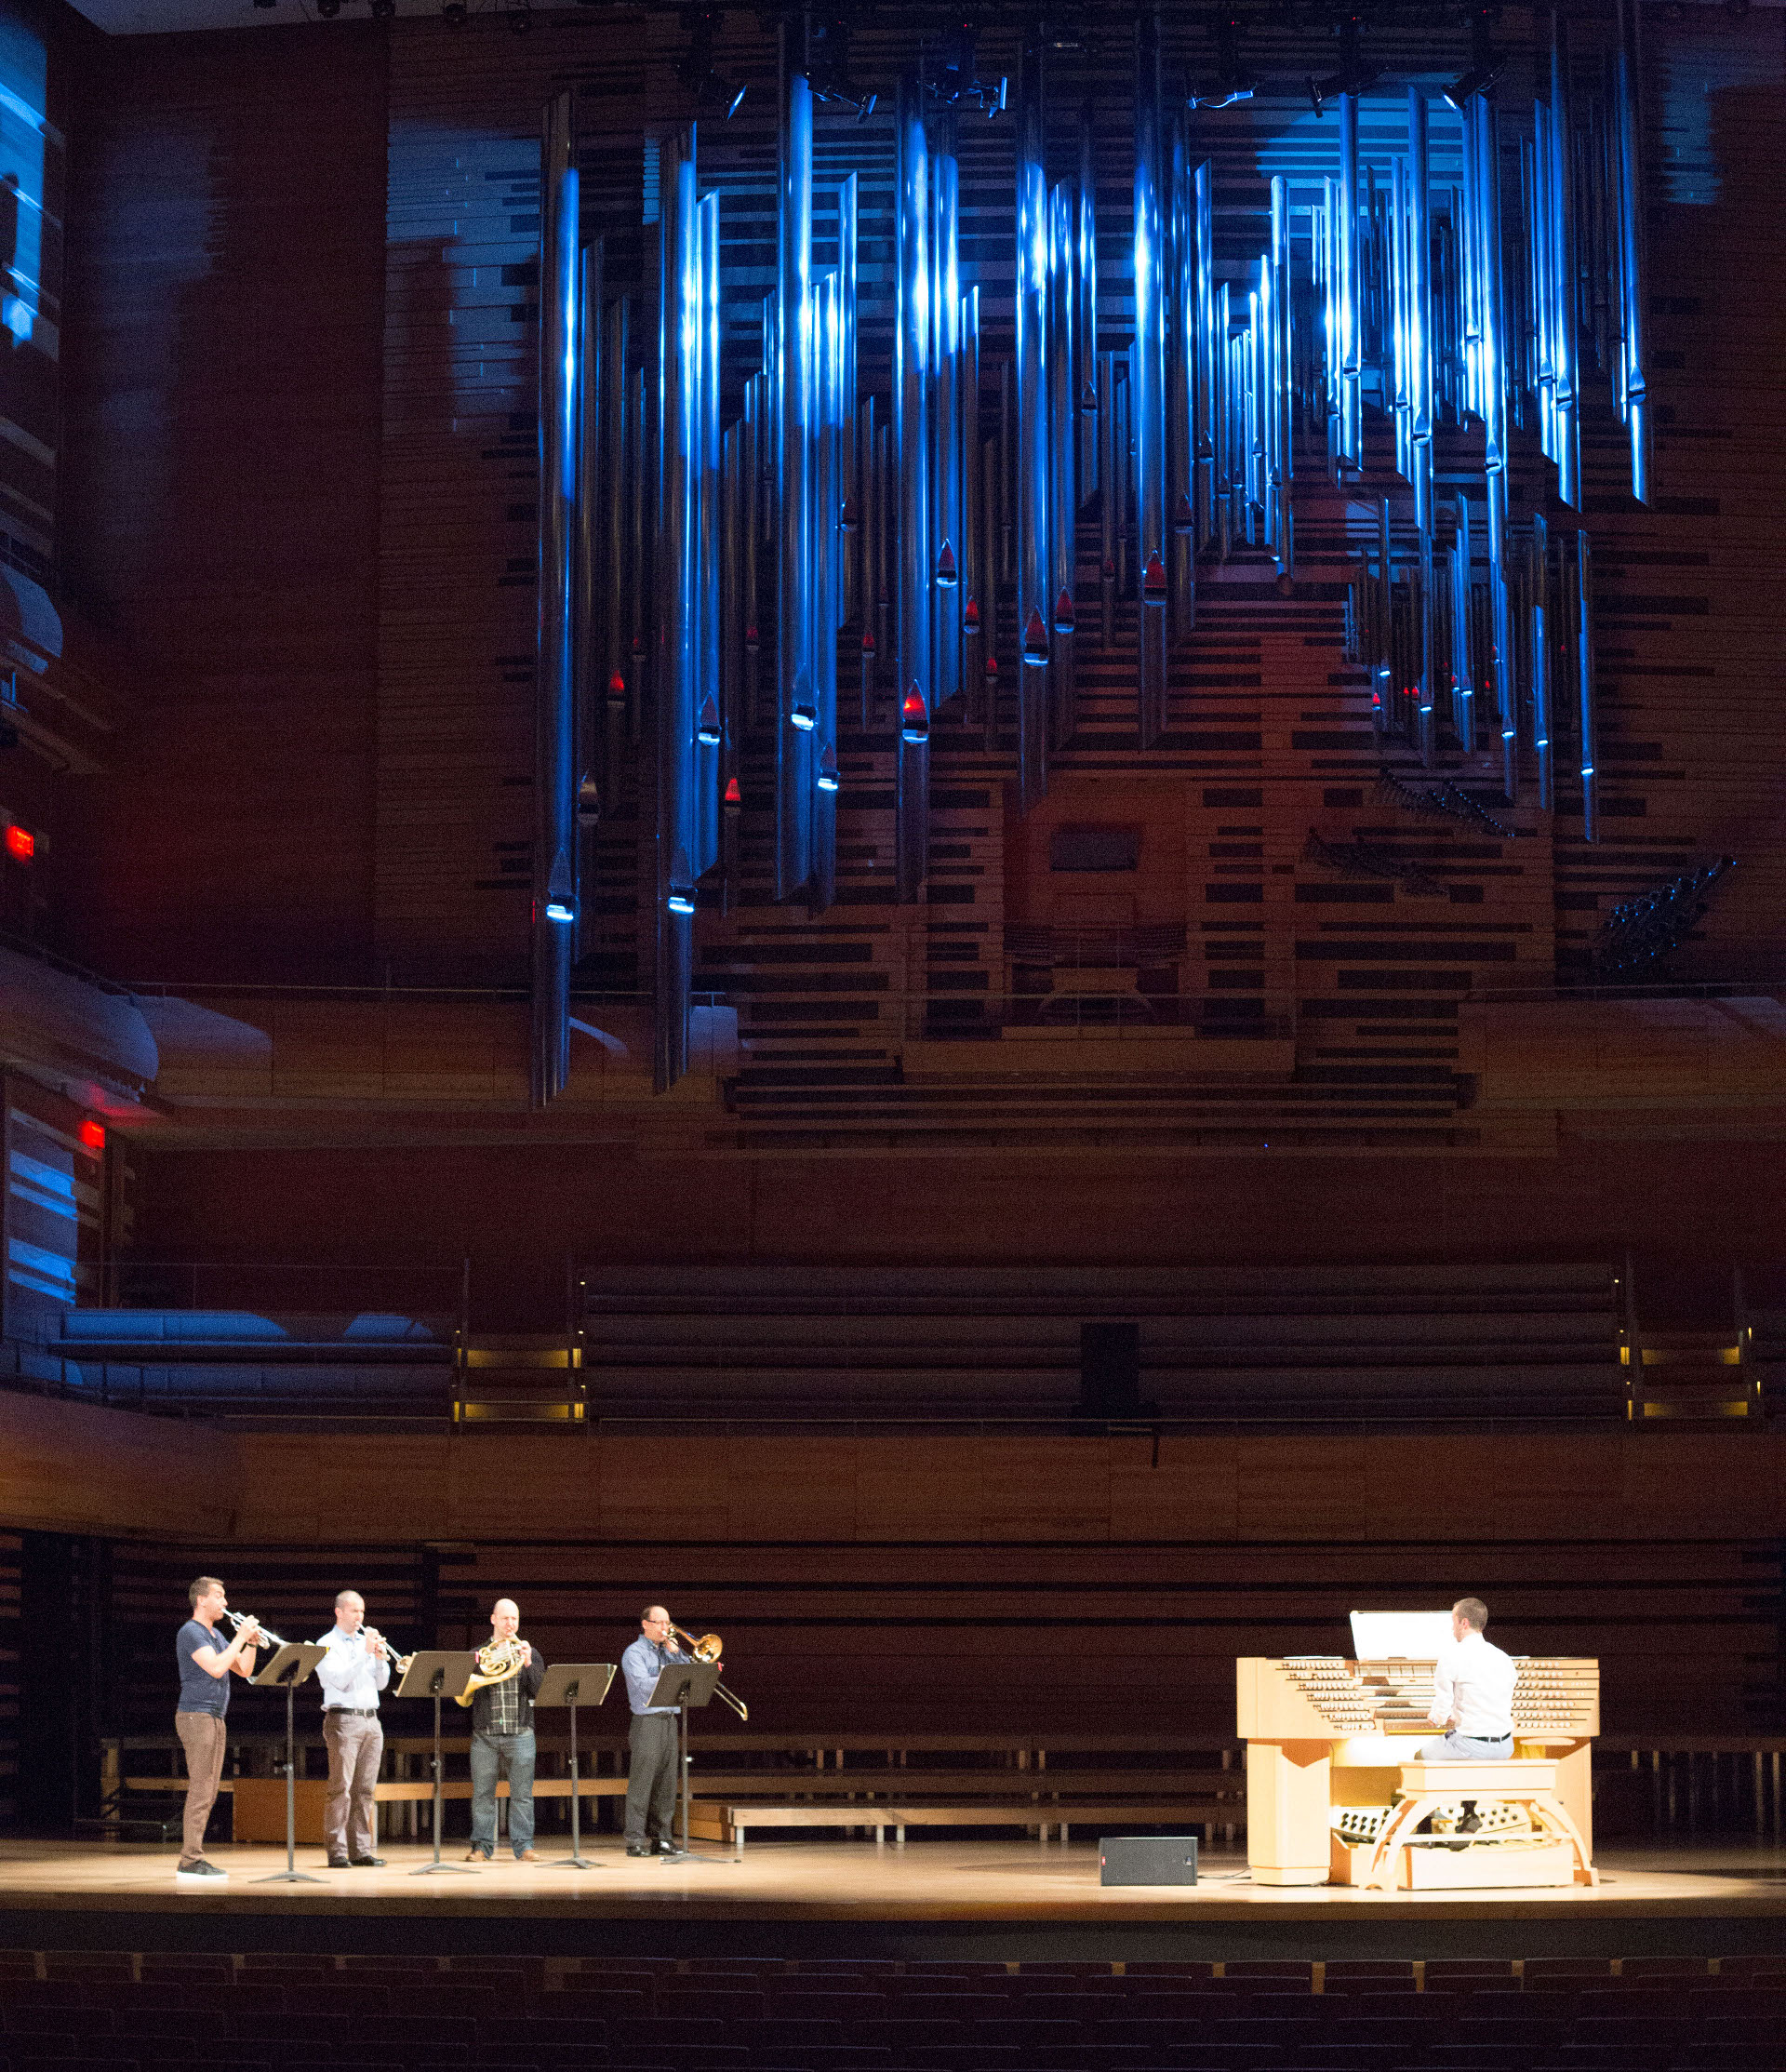
\includegraphics[width=\linewidth]{DressRehersal.jpg}
  \caption{The Pierre B\'{e}ique Organ in the OSM concert hall during
    a rehearsal on May 15th, 2015. Approximately 97\% of the organs'
    6489 pipes are out of sight behind the woodwork. Photo credit: Ben
    Bloomberg}
  \label{fig:le-corbusier-sketch}
\end{figure*}


%%% Local Variables:
%%% mode: latex
%%% TeX-master: "CharlesHolbrow_MAS_Thesis"
%%% End:
